\documentclass{article}

\usepackage{graphicx}
\usepackage[margin=1in]{geometry}
\usepackage{booktabs}
\usepackage{float}
\usepackage{amsmath}

\begin{document}

\title{Rotation-Invariant Composite Kernel Findings}
\author{}
\date{18 February 2026}
\maketitle

\section*{Questions}
\begin{itemize}
    \item Can we make the composed kernel rotation invariant using right-angle rotations?
    \item What is test-set performance after enforcing rotation invariance?
\end{itemize}

\section*{Method}
A rotation-invariant composite kernel was constructed from the best single composed kernel:
\[
K_{\text{RI}} = \frac{1}{4}\sum_{k=0}^{3} \operatorname{rot90}(K_{\text{comp}}, k)
\]
where $k \in \{0,1,2,3\}$ corresponds to $0^\circ, 90^\circ, 180^\circ, 270^\circ$.

\begin{itemize}
    \item trains a single-feature classifier on train patches using $K_{\text{RI}}$,
    \item evaluates on the original test split,
    \item evaluates again on $90^\circ$, $180^\circ$, and $270^\circ$ rotated versions of the same test patches.
\end{itemize}

\section*{Rotation-Invariant Kernel Visualization}
\begin{figure}[H]
    \centering
    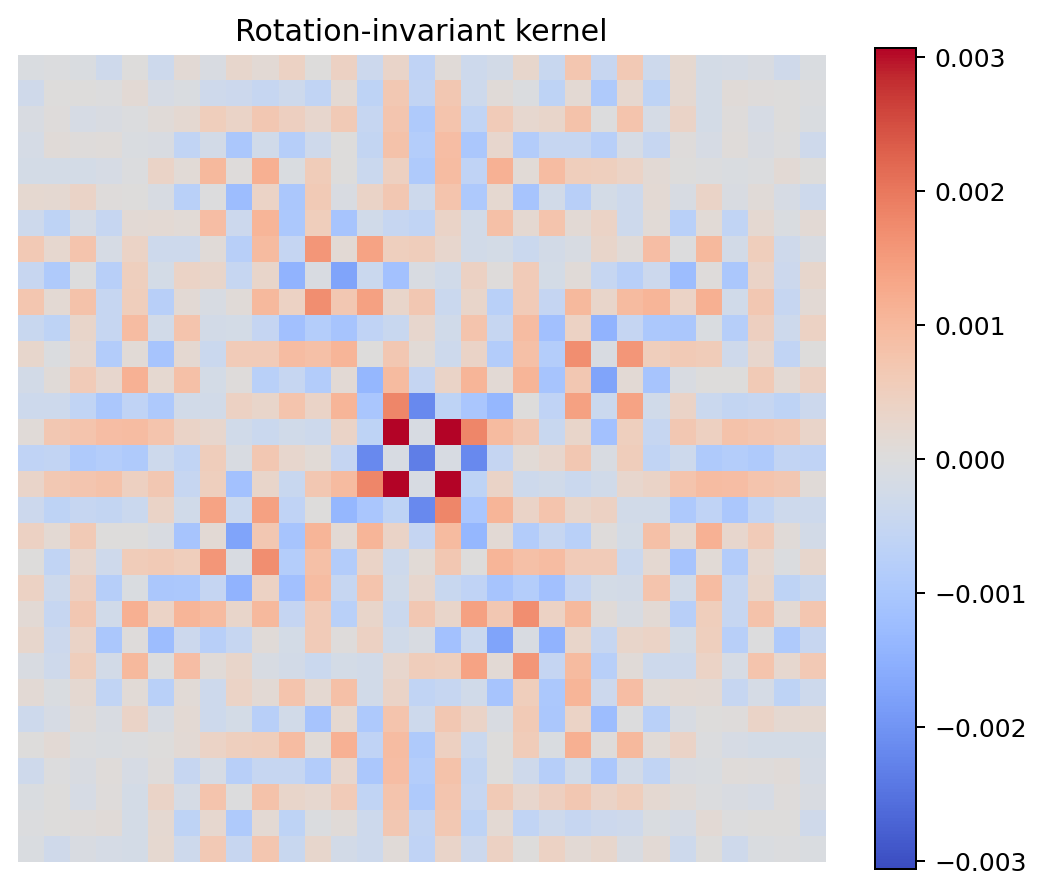
\includegraphics[width=0.85\linewidth]{../results/exp_022_mmr_nperFamily500_nComposition1250/rotation_invariant_kernel.png}
    \caption{Rotation-invariant composite kernel $K_{\text{RI}}$ used for the test-set evaluations.}
\end{figure}

\section*{Data and Model Setup}
\begin{itemize}
    \item Train split: $X_{\text{in}}=(2800,128,128)$, $X_{\text{out}}=(3000,128,128)$
    \item Test split: $X_{\text{in}}=(1040,128,128)$, $X_{\text{out}}=(830,128,128)$
    \item Test sample count: $N=1870$
    \item Classifier type from config: \texttt{logistic}
\end{itemize}

\section*{Results}
\begin{center}
\begin{tabular}{lcc}
\toprule
Evaluation & Test AUC & Test ACC \\
\midrule
Original invariant kernel (test $0^\circ$) & 0.890774 & 0.809091 \\
Invariant kernel, test rotated $90^\circ$ & 0.890774 & 0.809091 \\
Invariant kernel, test rotated $180^\circ$ & 0.890774 & 0.809091 \\
Invariant kernel, test rotated $270^\circ$ & 0.890773 & 0.809091 \\
\bottomrule
\end{tabular}
\end{center}

\vspace{0.5em}
\textbf{Rotation deltas (rotated $-$ original invariant kernel):}
\begin{itemize}
    \item $90^\circ$: $\Delta$AUC $= +0.000000$, $\Delta$ACC $= +0.000000$
    \item $180^\circ$: $\Delta$AUC $= +0.000000$, $\Delta$ACC $= +0.000000$
    \item $270^\circ$: $\Delta$AUC $= -0.000001$, $\Delta$ACC $= +0.000000$
\end{itemize}

\section*{Findings}
\begin{itemize}
    \item The averaging construction produced a kernel that is effectively right-angle rotation invariant in evaluation.
    \item Test accuracy is exactly unchanged across $0^\circ$, $90^\circ$, $180^\circ$, and $270^\circ$.
    \item Test AUC is also stable, with only a negligible numerical difference at $270^\circ$ ($-10^{-6}$).
\end{itemize}

\section*{Work in Progress}
\begin{itemize}
    \item \textbf{Smarter kernel sampling:} replacing purely random parameter sampling with low-discrepancy strategies such as QMC or Latin Hypercube Sampling to improve coverage of each family parameter space.
    \item \textbf{Per-family normalization:} applying normalization rules tailored to each kernel family before composition and response extraction, to better balance family-specific amplitude and scale differences.
\end{itemize}

\section*{Conclusion}
The rotation-invariant composite kernel achieved stable test performance across all right-angle rotations in this run. The invariance objective was met on the test set.

\end{document}
